%%%%%%%%%%%%%%%%%%%%%%%%%%%%%%%%%%%%%%%%%
% Beamer Presentation
% LaTeX Template
% Version 1.0 (10/11/12)
%
% This template has been downloaded from:
% http://www.LaTeXTemplates.com
%
% License:
% CC BY-NC-SA 3.0 (http://creativecommons.org/licenses/by-nc-sa/3.0/)
%
%%%%%%%%%%%%%%%%%%%%%%%%%%%%%%%%%%%%%%%%%

%----------------------------------------------------------------------------------------
%	PACKAGES AND THEMES
%----------------------------------------------------------------------------------------

\documentclass{beamer}

\mode<presentation> {
	
	% The Beamer class comes with a number of default slide themes
	% which change the colors and layouts of slides. Below this is a list
	% of all the themes, uncomment each in turn to see what they look like.
	
	%\usetheme{default}
	%\usetheme{AnnArbor}
	%\usetheme{Antibes}
	%\usetheme{Bergen}
	%\usetheme{Berkeley}
	%\usetheme{Berlin}
	%\usetheme{Boadilla}
	%\usetheme{CambridgeUS}
	%\usetheme{Copenhagen}
	%\usetheme{Darmstadt}
	%\usetheme{Dresden}
	%\usetheme{Frankfurt}
	%\usetheme{Goettingen}
	%\usetheme{Hannover}
	%\usetheme{Ilmenau}
	%\usetheme{JuanLesPins}
	%\usetheme{Luebeck}
	\usetheme{Madrid}
	%\usetheme{Malmoe}
	%\usetheme{Marburg}
	%\usetheme{Montpellier}
	%\usetheme{PaloAlto}
	%\usetheme{Pittsburgh}
	%\usetheme{Rochester}
	%\usetheme{Singapore}
	%\usetheme{Szeged}
	%\usetheme{Warsaw}
	
	% As well as themes, the Beamer class has a number of color themes
	% for any slide theme. Uncomment each of these in turn to see how it
	% changes the colors of your current slide theme.
	
	%\usecolortheme{albatross}
	\usecolortheme{beaver}
	%\usecolortheme{beetle}
	%\usecolortheme{crane}
	%\usecolortheme{dolphin}
	%\usecolortheme{dove}
	%\usecolortheme{fly}
	%\usecolortheme{lily}
	%\usecolortheme{orchid}
	%\usecolortheme{rose}
	%\usecolortheme{seagull}
	%\usecolortheme{seahorse}
	%\usecolortheme{whale}
	%\usecolortheme{wolverine}
	
	%\setbeamertemplate{footline} % To remove the footer line in all slides uncomment this line
	%\setbeamertemplate{footline}[page number] % To replace the footer line in all slides with a simple slide count uncomment this line
	
	%\setbeamertemplate{navigation symbols}{} % To remove the navigation symbols from the bottom of all slides uncomment this line
}

\usepackage{graphicx} % Allows including images
\usepackage{subfigure}
\usepackage{booktabs} % Allows the use of \toprule, \midrule and \bottomrule in tables
\usepackage{bm}

%----------------------------------------------------------------------------------------
%	TITLE PAGE
%----------------------------------------------------------------------------------------

\title[BFA]{Sparse Bayesian infinite factor models} 

\author{Ganchao Wei} 
\date{October 27, 2021}

\begin{document}
	
	\begin{frame}
		\titlepage % Print the title page as the first slide
	\end{frame}
	
	\begin{frame}
		\frametitle{Overview} % Table of contents slide, comment this block out to remove it
		\tableofcontents
	\end{frame}
	
	%--------------------------------------------------------------------
	%	PRESENTATION SLIDES
	%--------------------------------------------------------------------
	
	\section{Introduction}
	
	\begin{frame}
		\frametitle{Introduction}
		The generic form of a latent factor model:
		$$y_i = \Lambda \eta_i + \epsilon_i$$
		, where $y_i \in \mathbb{R}^p$, $\Lambda \in \mathbb{R}^{p \times k}$, $\eta_i \sim N_k(9, I_k)$, $\epsilon_i \sim N_p(0, \Sigma)$ and $\Sigma = diag(\sigma_1^2,\ldots, \sigma_p^2)$. Therefore, marginally, $y_i \sim N_p(0, \Omega)$ with $\Omega = \Lambda \Lambda^{T} + \Sigma$	.\\
		\vspace{\baselineskip}
		In traditional factor analysis, we need to put constraints on loading. However, from Bayesian perspective, one does not require identifiability of the loading elements for a wide class of applications.  By making use of this, they define the prior on a parameter-expanded loadings matrix with redundant parameters, resulting in better computational properties while simplifying the theory.
	\end{frame}
	
	\section{Prior Specification}
	\begin{frame}
		\frametitle{Prior Specification}
		Prior for $\Sigma$: usual inverse gamma priors on the diagonal elements.\\
		\vspace{\baselineskip}
		Denote $\Lambda = (\lambda_{jh})$, for $j=1,\ldots,p$ and $h=1,\ldots,\infty$. The entries of $\Lambda$ decrease in magnitude as the column index increases, without any restrictions. More specifically, they use a shrinkage-type prior with the degree of shrinkage increasing across the column index as follows,
		\begin{figure}
			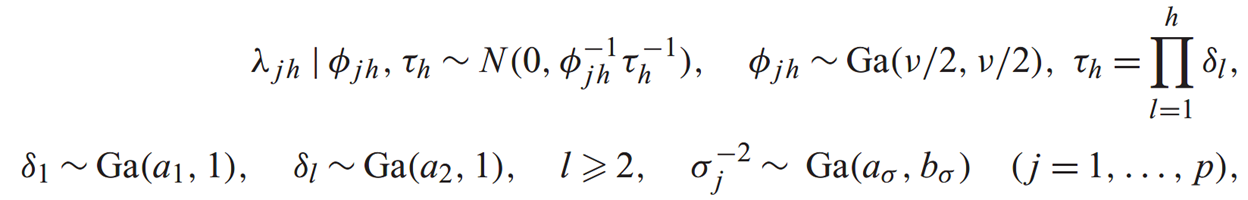
\includegraphics[width=0.9\linewidth]{image001.png}
		\end{figure}
		
	\end{frame}
	
	
	\begin{frame}
		\frametitle{Prior Specification}
		\begin{figure}
			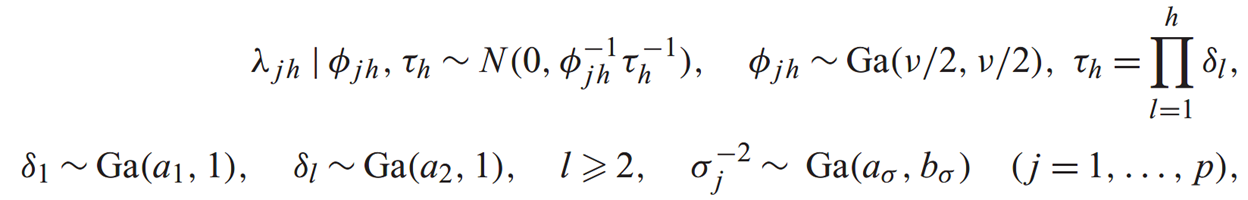
\includegraphics[width=0.9\linewidth]{image001.png}
		\end{figure}
		\begin{itemize}
			\item 
			$\delta_l (l=1,\ldots,\infty,)$ are independent
			\item
			$\tau_h$ is a global shrinkage parameter
			\item
			$\phi_{jh}s$ are local shrinkage parameters
			\item
			$\tau_h$ are stochatially increasing under the restriction $a_2 >1$
		\end{itemize}
	For the shrinkage prior, we can show the weak consistency of posterior and the prior is free of order dependence.\\
	\vspace{\baselineskip}
	They further place gamma priors on $a_1$ and $a_2$ to learn these key hyperparameters from the data.
	\end{frame}
	
	\section{Posterior Computation}
	\begin{frame}
		\frametitle{Gibbs sampler with a fixed truncation level}
		After truncating the loading matrix to have $k^* \ll p$
		\begin{figure}
			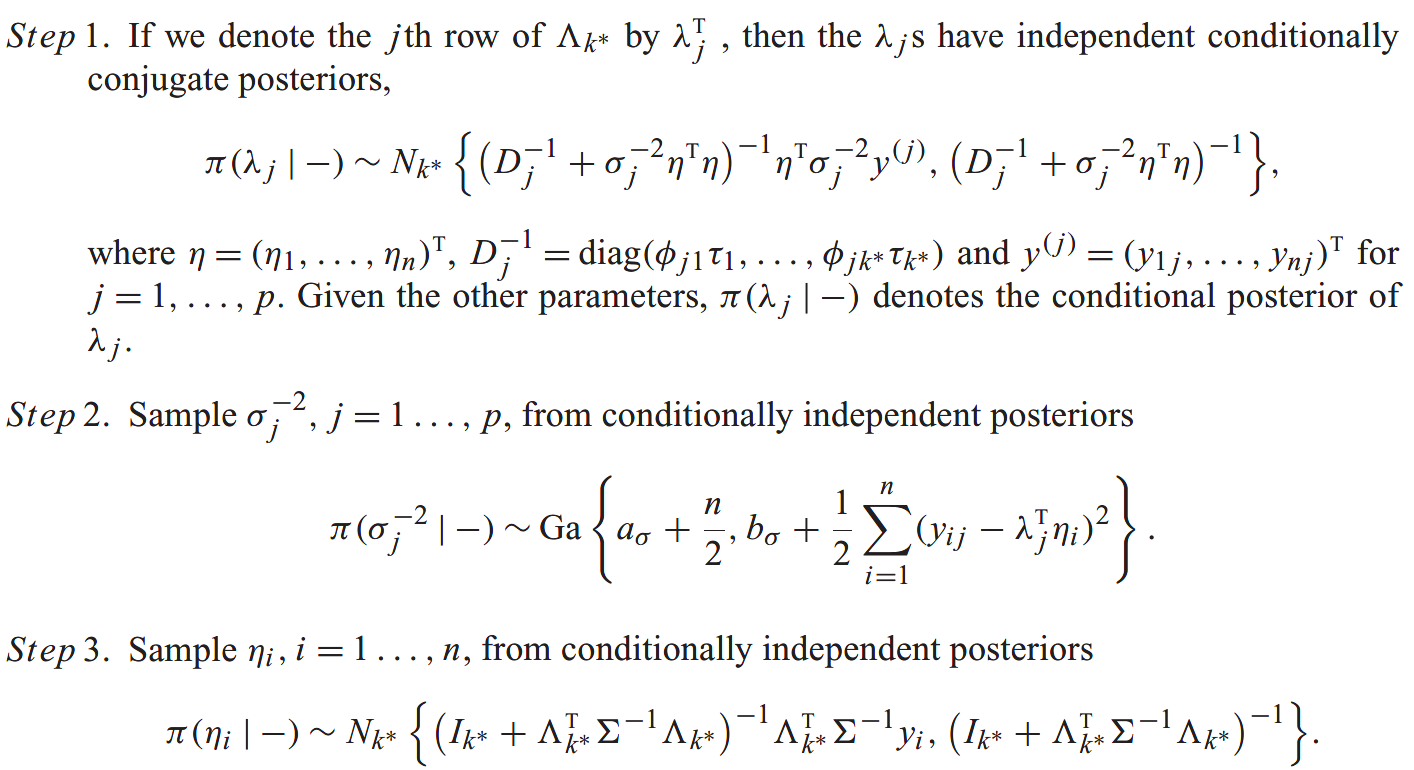
\includegraphics[width=0.9\linewidth]{image002.png}
		\end{figure}
	\end{frame}
	
	
	\begin{frame}
		\frametitle{Gibbs sampler with a fixed}
		\begin{figure}
			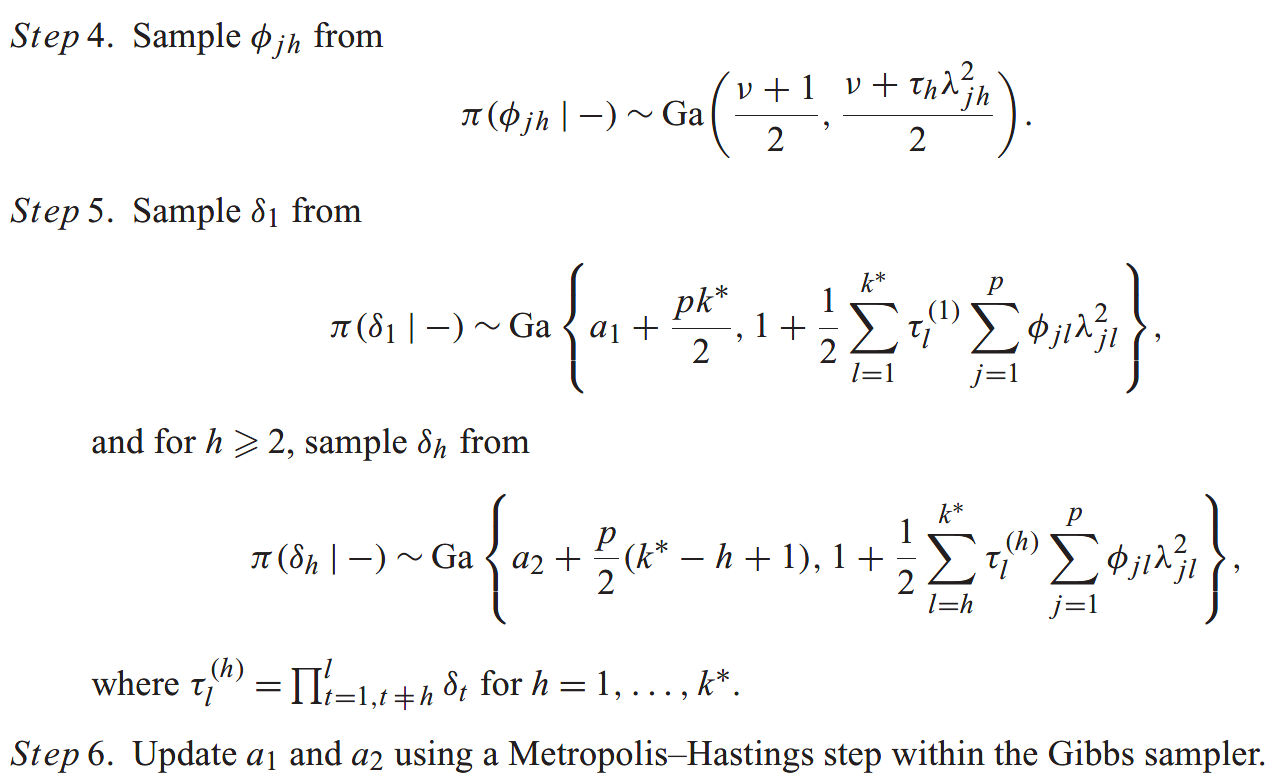
\includegraphics[width=0.9\linewidth]{image003.png}
		\end{figure}	
	\end{frame}
	
	\begin{frame}
		\frametitle{Choosing the number of factors adaptively}
		Do it with adaptive Gibbs sampler: tune the number of factors as the sampler progresses.
		\begin{itemize}
			\item 
			adapt with probability $p(t) = exp(\alpha_0 + \alpha_1 t)$ at the $t$th iteration
			\item
			$\alpha_0$ and $\alpha_1$ are chosen so that adaptation occurs around every 10 iterations at the beginning of the chain, but decreases in frequency exponentially fast.
			\item
			Generate $u_t \sim U(0,1)$. If $u_t \leq p(t)$, monitor the columns in the loadings having all elements within some pre-specified small neighborhood of 0.
			\item
			if the number of such columns drops to 0 $\Rightarrow$ generate new column from prior
			\item
			Otherwise, discard the redundant columns.
			
		\end{itemize}
	\end{frame}
	
	\section{Simulation Example}
	
	\begin{frame}
		\frametitle{Factor selection and covariance matrix estimation}
		Simulation settings:
		\begin{itemize}
			\item 
			$y_i \in \mathbb{R}^p$ for $i=1,\ldots,200$. The diagonal elements of $\Sigma^-1$ are drawn independently from Ga(1, 0.25).
			\item
			They choose 3 combinations of (p,k): (100,5), (500, 10) and (1000, 15)
			\item
			For each pair, there are 50 simulation replicates
			\item
			25000 iterations with 5000 burn-in, and collect every 5th sample to thin the chain
			\item
			3 methods are compared: (1) the proposedmethod MGPS, (2) banding sample covariance and (3) EM for MAP.
		\end{itemize}
	\end{frame}
	
	\begin{frame}
		\frametitle{Factor selection and covariance matrix estimation}
		\begin{figure}
			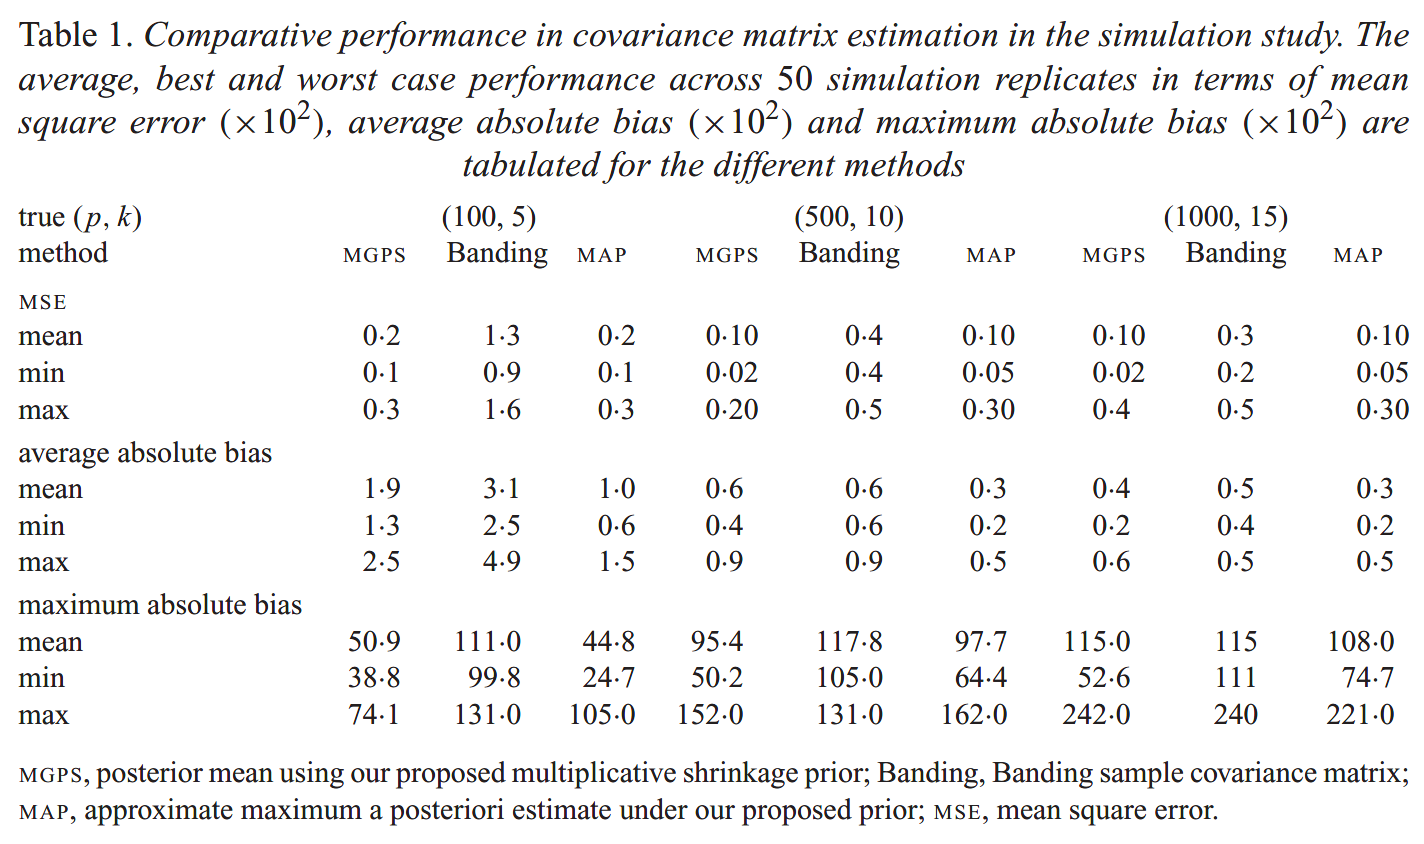
\includegraphics[width=0.9\linewidth]{image004.png}
		\end{figure}
	\end{frame}
	
	\begin{frame}
		\frametitle{Latent factor regression}
		Instead of doing regularization (e.g. LASSO \& elastic net), we can regard it as the latent factor regression problem.\\
		Consider $E(z_i|x_i) = x_i^T\beta$, with $\beta = \Omega_{xx}^{-1}\Omega_{zx}$ and $\Omega_{xx} = \Lambda_x\Lambda_x^T + \Sigma_{xx}$. Just use the sub-blocks of factor analysis results, then everything is done. 
		\begin{figure}
			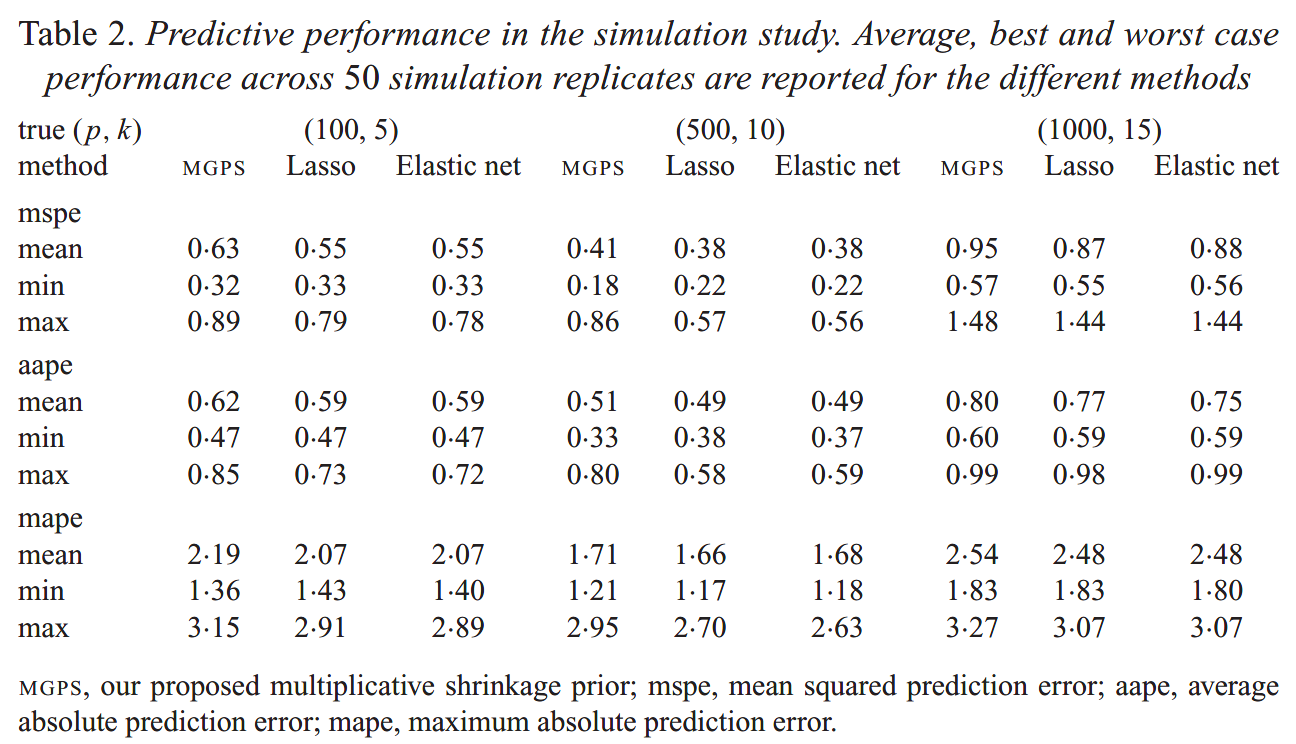
\includegraphics[width=0.8\linewidth]{image005.png}
		\end{figure}
	\end{frame}
	
	\begin{frame}
		\frametitle{Latent factor regression}
		\begin{figure}
			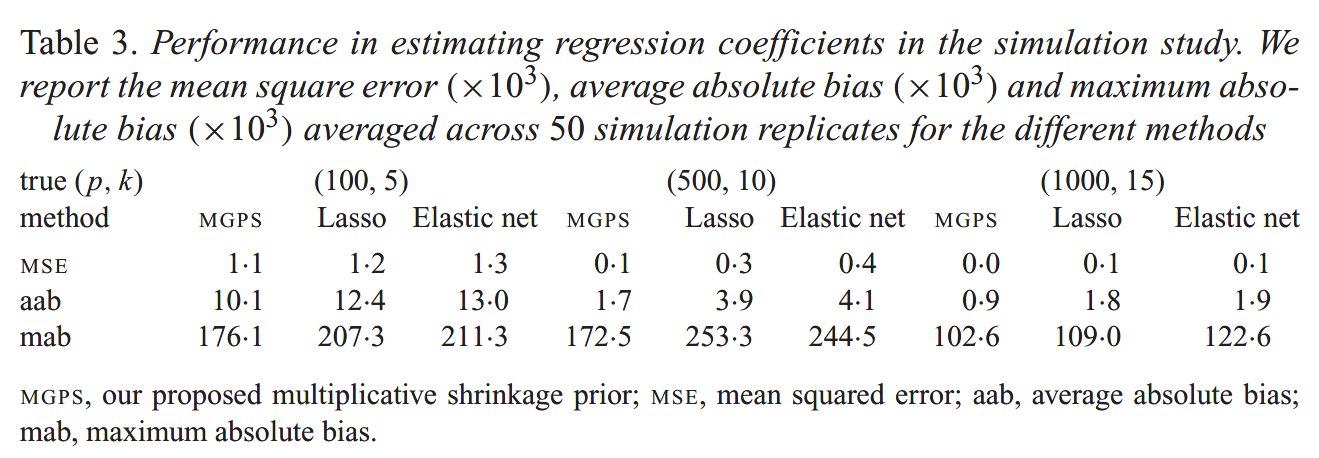
\includegraphics[width=0.8\linewidth]{image006.png}
			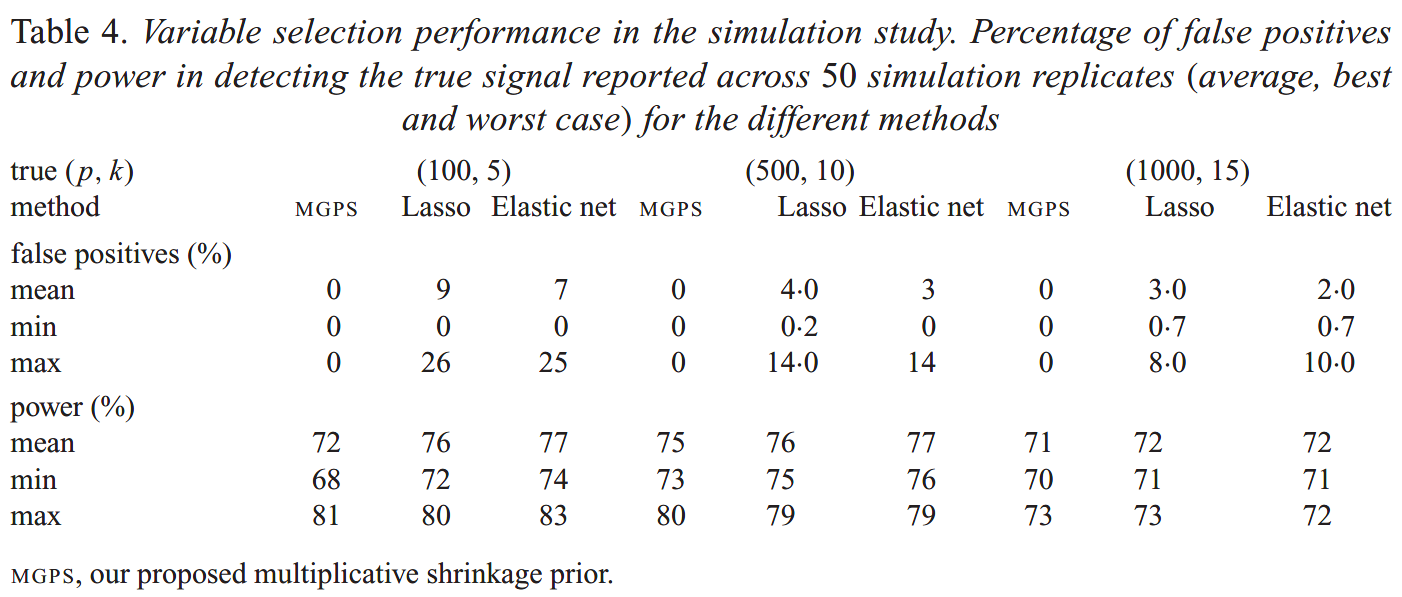
\includegraphics[width=0.8\linewidth]{image007.png}
		\end{figure}
	\end{frame}
	
	\section{Application}
	\begin{frame}
		\frametitle{Diffuse Large-B-Cell Lymphoma Application}
		\textbf{Goal}: (1) simultaneously identifying important features and (2) obtain a predictive model for the exact survival times.\\
		\begin{itemize}
			\item 
			Let $T_i$ denote the survival time for $i$th patient and let $x_i$ denote the corresponding 7399 dimensional feature vector, for $i=1,\ldots,72$.
			\item
			Combine all the data into $y_i = (z_i, x_i^T)^T$ and $z_i =\log(1+T_i)$
			\item
			Then do latent factor regression as in simulation example.
		\end{itemize}
		After fitting the model, they find 17 features, which matches previous results.
	\end{frame}
	
	
	
	
\end{document}